\chapter{Sistema de Video}\label{image}

\vspace{-0.5cm}

\section*{Configuração Câmera}

Para a realização dos filmes os passos a seguir são:

\begin{enumerate}
\item Ligue a câmera e verifique que o cartão de memória esteja vazio. %Para isto tem que ir ao menu e escolher com o cursor a terceira opção como é mostrado na Figura~\ref{fig:camera}-A. Uma vez no menu com o cursor da esquerda escolha a opção ``Apagar", dê ``OK" quantas vezes seja necessário para apagar as fotos e filmes do cartão de memória.

\item Configure a câmera para a realização do filme. 
\begin{itemize}
\item Para a câmera Olympus: %Entre no menu e escolha a segunda opção como indicado na Figura~\ref{fig:camera}-B.  A configuração escolhida deve ser: 
\begin{enumerate}
\item {\bf Tamanho De Imag} VGA
\item {\bf Imagens Por Seg.} 15 ou 30 fas (fotos por segundo) 
\item {\bf Microfone} Desl.  (desligado)
\item {\bf Modo AF}: configure a câmera para que sempre faça foco no objeto de interesse, mesmo quando ele esteja em movimento. Novamente, entre no menu e escolha a primeira opção como indicado na Figura~\ref{fig:camera}-C. No menu da esquerda escolha a terceira opção ``Modo AF" e logo ``Rastreia AF". Dê ``OK"  e pressione o botão do menu para sair do mesmo.
\end{enumerate}

\item Para a câmera Nikon Coolpix s3600, aperte o botão ``Menu", selecione o ícone de câmera de vídeo conforme a Figura~\ref{fig:nikon} e selecione:
\begin{enumerate}
\item {\bf Opções de vídeo}: 480/30p
\item {\bf Modo foco automático:} AF-F AF constante
\item {\bf VR do vídeo}: desligado
\end{enumerate}
\item Para a câmera Sony Cyber-shot, aperte o botão ``Menu" e busque as opções a seguir, conforme a Figura~\ref{fig:sony}: 
\begin{enumerate}
\item {\bf Tamanho Filme:} VGA
\item {\bf ACT:} STD movimentação moderada (nem todas as câmeras tem essa opção no menu à esquerda, com um ícone de mão)
\end{enumerate}
\end{itemize} 
\end{enumerate}

Desta forma sua câmera está configurada e você pode começar a fazer sua aquisição de dados. 
\begin{figure}[t!]
\begin{center}
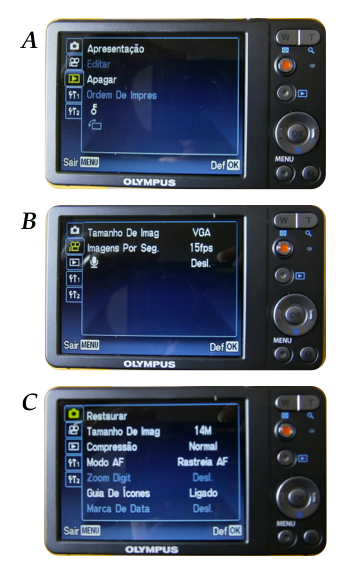
\includegraphics[width=9cm]{fig/CameraOlympus.png}
\caption{\label{fig:camera} Configuração da câmera Olympus.}
\vspace{-0.5cm}
\end{center}
\end{figure}

\begin{figure}[h!]
\begin{center}
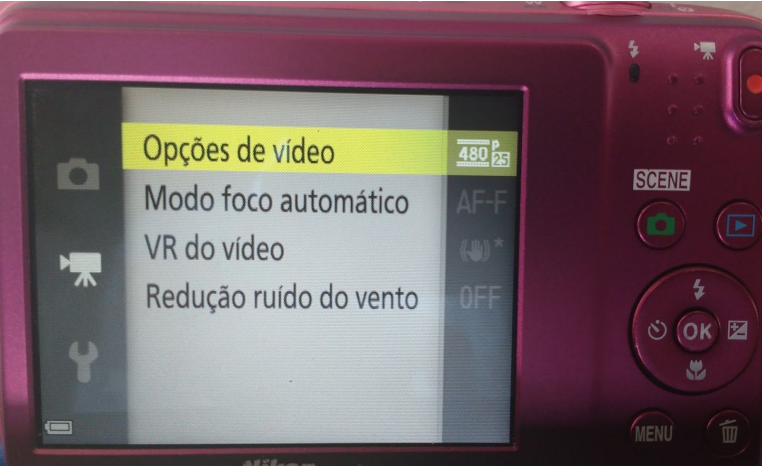
\includegraphics[width=9cm]{fig/cameraNikon.png}
\caption{\label{fig:nikon} Configuração da câmera Nikon.}
\vspace{-0.5cm}
\end{center}
\end{figure}

\begin{figure}[h!]
\begin{center}
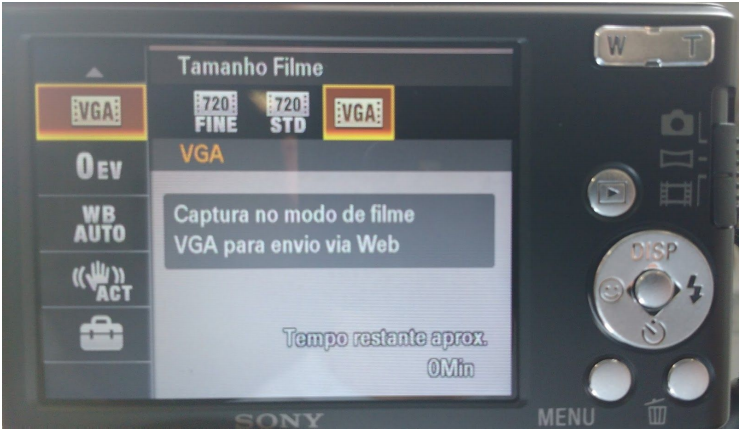
\includegraphics[width=9cm]{fig/cameraSony.png}
\caption{\label{fig:sony} Configuração da câmera Sony.}
\vspace{-0.5cm}
\end{center}
\end{figure}
\newpage
\section*{Leitura manual da posição do carrinho}
\begin{enumerate}

\item Uma vez registrado o movimento do carrinho com a câmera proceda a baixar o filme que você fez numa pasta no desktop do seu computador chamada MRU. Para algumas câmeras, o video é salvo no formato MP4 e precisa ser convertido em AVI para análise no programa ImageJ. Um tutorial para conversão dos videos encontra-se nas bancadas, próximo ao computador.
\item Abra o programa ImageJ.
\item No ImageJ abra o filme que você fez em formato AVI. Aparecerá uma tela com algumas indicações como se mostra na Figura~\ref{fig:frame}, “First Frame 1”, “Last Frame 135”, que podem em princípio ser alteradas pelo usuário. Essas informações correspondem ao número de imagens contidas no filme e permitem que escolhamos apenas algumas delas para serem exibidas. Mantenha como está e tecle “Ok”.
\begin{figure}[t!]
\begin{center}
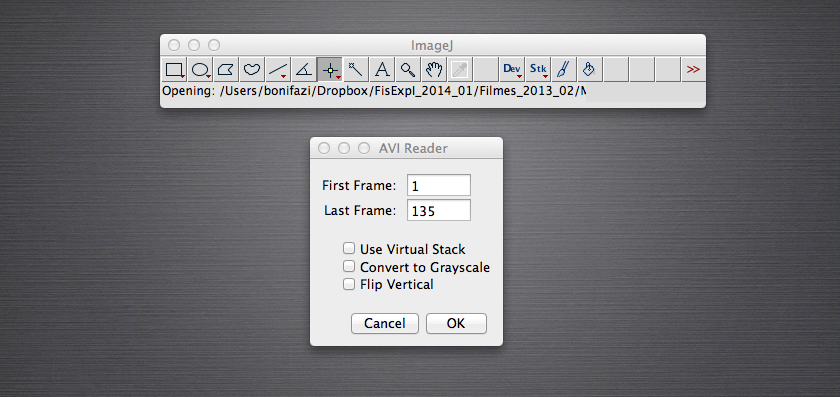
\includegraphics[width=11cm]{fig/frame}
\caption{\label{fig:frame} ImageJ: tela de inicio para carregar o filme.}
%\vspace{-0.5cm}
%\end{center}
%\end{figure}
%\begin{figure}[h]
%\begin{center}
\vspace{0.3cm}
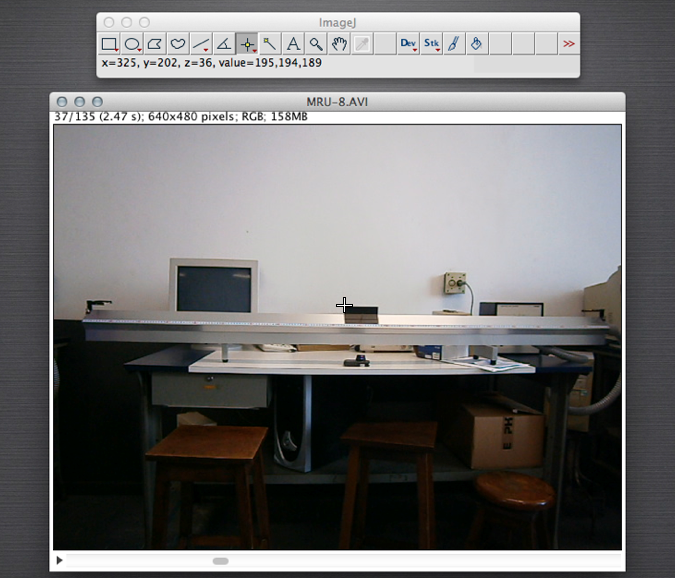
\includegraphics[width=11cm]{fig/cursor}
\caption{\label{fig:exMovie} ImageJ: posição do cursor sobre a imagem.}
\vspace{-0.6cm}
\end{center}
\end{figure}

\item Após o filme aberto você pode escolher a ferramenta de “zoom” que fica na barra de ferramentas do programa para ver melhor as imagens. A resolução das imagens não é muito boa, mas não precisamos mais do que isso para fazer a análise do experimento.
\item Experimente passar o cursor do mouse sobre a imagem. Você verá que embaixo da barra de ferramentas do ImageJ aparecerão alguns números, por exemplo, na Figura~\ref{fig:exMovie}: x=325, y=202, z=36, value = 195. As letras “x” e “y” correspondem à posição do cursor em “pixels” no sistema de referência mostrado na Figura~\ref{fig:exMovie}. A letra “z” corresponde à ordem em que imagem foi capturada em relação ao início do filme. Finalmente, “value” corresponde aos níveis de vermelho, verde e azul da imagem, nesta ordem. Para as análises que faremos, só utilizaremos a posição “x e y” do cursor.
\item Observe agora no canto superior esquerdo das imagens do filme (Figura~\ref{fig:exMovie}). Aparecem números semelhantes a “37/135 (2.47s); 640x480 pixels; RGB; 158 MB”. O primeiro deles significa que está sendo exibida a imagem 37 de um total de 135. O instante de tempo no qual essa imagem foi capturada em relação ao início do filme é indicado pelo número entre parênteses “2.47s” que é dado por $1/15 \times 37$~s (onde 1/15 corresponde a 15 fotos ou {\it frames}  por segundo), “640 X 480 pixels” corresponde às dimensões da imagem em número de “pixels”, “RGB” corresponde à qualidade da imagem, e “158 MB” corresponde ao espaço de memória do computador que foi utilizado para guardar o filme. Para nossas análises o número importante dentre esses é o que corresponde ao número de imagem e ao instante de tempo em que a imagem foi capturada. \underline{Observação}: estes números serão diferentes para cada filme.
\end{enumerate}


\section*{Rotação do Filme}

Para realizar a análise dos dados, é necessário que a medida do deslocamento do carrinho seja apenas em uma dimensão, por exemplo, na horizontal.  Se o eixo horizontal da câmera não está bem alinhado com o trilho, precisamos realizar uma rotação do filme antes de proceder à leitura da posição do carrinho. Portanto, o primeiro passo é a determinação do ângulo de rotação.  A mesma pode ser realizada de duas formas diferentes:

\vspace{-0.7cm}
\subsection*{\underline{Forma manual}}
\vspace{-0.2cm}
\begin{enumerate}
\item Determine com os cursores as coordenadas ``x e y" das extremidades do trilho, tendo desta forma $(x_1,y_1) e (x_2, y_2)$ como se mostra na figura~\ref{fig:coord}.
\item Utilizando trigonometria, e utilizando uma calculadora, determine o ângulo de inclinação como o $\arctan{(y_2-y_1)/(x_2-x_1)}$. \underline{Observação:} o ângulo tem que ser determinado em graus.
\end{enumerate}

\vspace{-0.9cm}
\subsection*{\underline{Forma automática}}
\vspace{-0.2cm}
\begin{enumerate}
\item Escolha o botão de “\^Angulo” (círculo na Figura~\ref{fig:angulo}-A), que fica na barra de ferramentas do programa ImageJ para poder marcar o ângulo que quer ser determinado. 
\item Movimente o cursor para marcar os três pontos que vão determinar o ângulo que o trilho forma com a horizontal (linhas cheias sobre o filme na Figura~\ref{fig:angulo}-B). Faça click cada vez que esteja na posição desejada.
\item Escolha a opção "Analyze" do menu principal e "Measure" do sub-menu.
\item O resultado será mostrado em uma outra janela (Figura~\ref{fig:angRes}), entre os quais estará o valor do ângulo desejado em graus.

\begin{figure}[t!]
\begin{center}
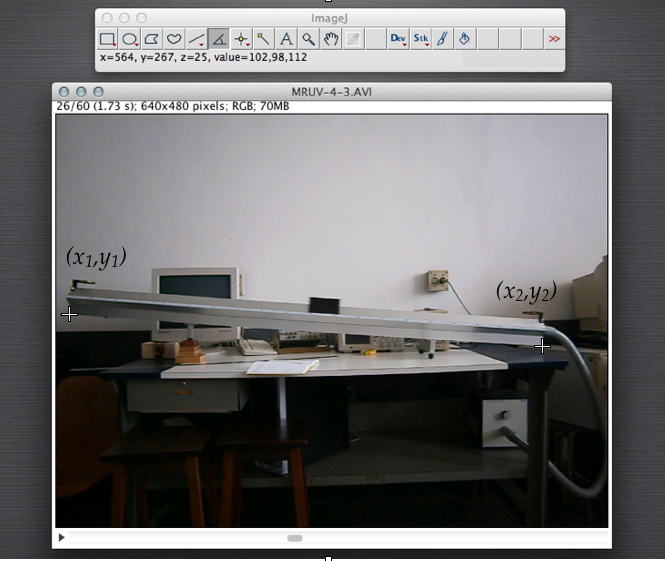
\includegraphics[width=9cm]{fig/coordman}
\caption{\label{fig:coord} ImageJ: determinação das coordenadas $(x_1,y_1) e (x_2, y_2)$, ver texto.}
\vspace{0.5cm}
%\end{center}
%\end{figure}
%\begin{figure}[h]
%\begin{center}
%\vspace{-0.3cm}
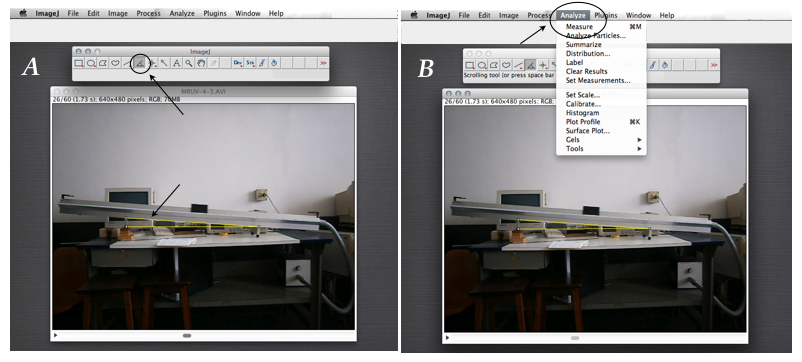
\includegraphics[width=16cm]{fig/AnguloAuto}
\caption{\label{fig:angulo} ImageJ: determinação do ângulo de inclinação do trilho, ver texto.}
\vspace{-0.5cm}
\end{center}
\end{figure}

Uma vez determinado o ângulo, devemos proceder a realizar a rotação do Filme. Para isto, deve seguir os seguintes passos: 
\begin{enumerate}
\item Escolha a opção ``Imagem" do menu principal, logo ``Transform" e finalmente ``Rotate", como mostrado na Figura~\ref{fig:rotate}-A.
\item Uma nova janela será aberta onde deve-ser informado o valor do ângulo de rotação, no nosso exemplo, o mesmo é de 4,101 graus (Figura~\ref{fig:angRes}). Este ângulo deve ser informado com o sinal negativo ($-$) se queremos realizar uma rotação no sentido anti-horário ou com sinal positivo ($+$) se a rotação é no sentido horário.
\item {\bf Como a rotação é uma ação definitiva} e não pode ser refeita, utilizar sempre o ``Preview" para poder ter certeza de que se está realizando a rotação desejada (ver Figura~\ref{fig:rotate}-B) antes de dar o ``OK" final.
\end{enumerate}

\begin{figure}[h!]
\begin{center}
\vspace{0.3cm}
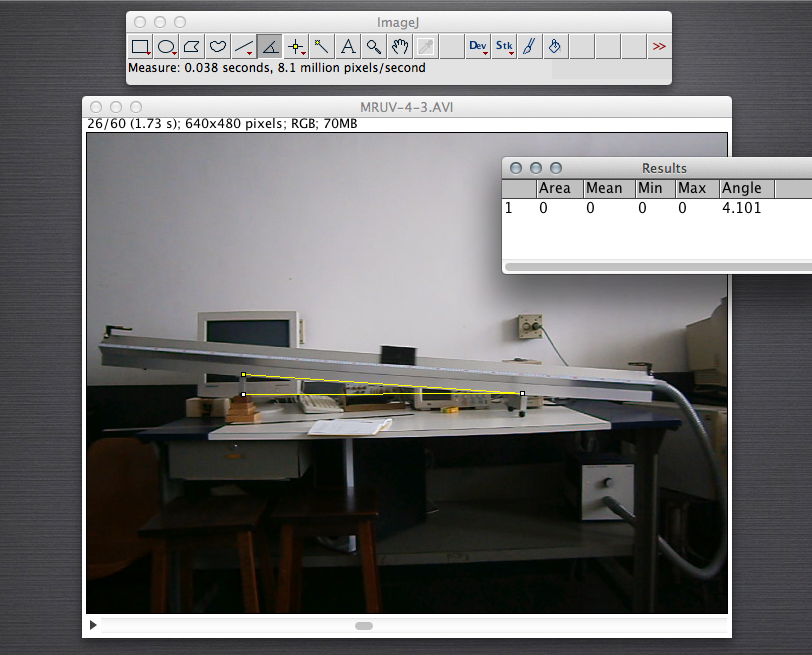
\includegraphics[width=10cm]{fig/AnguloResultado}
\caption{\label{fig:angRes} ImageJ: valor do ângulo de inclinação do trilho}
\vspace{0.5cm}
%\end{center}
%\end{figure}
%\begin{figure}[h]
%\begin{center}
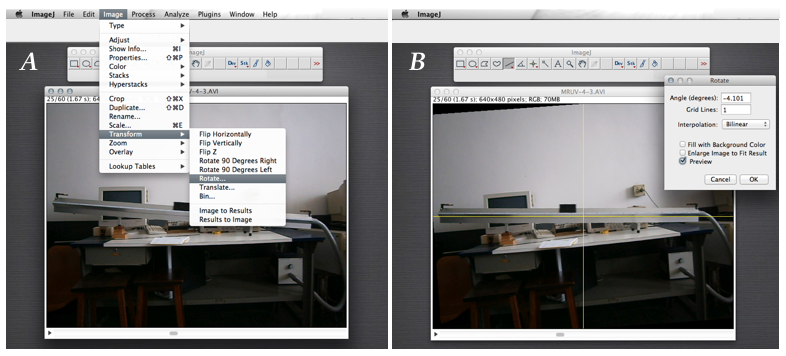
\includegraphics[width=16cm]{fig/Rotate}
\caption{\label{fig:rotate} ImageJ: rotação do filme por um determinado ângulo, ver texto}
\vspace{-0.5cm}
\end{center}
\end{figure}
\end{enumerate}
